% !TEX encoding = UTF-8 Unicode 
% !TeX spellcheck = pl_PL
% http://wiki.languagetool.org/checking-la-tex-with-languagetool
\documentclass{dyplom}
\usepackage[utf8]{inputenc}
\usepackage{hyperref}
%%
\usepackage{lipsum}

% Dane o pracy
\author{Anna Nowak}
\title{Kot Ali a Docker}
\titlen{The Ala's cat and the Docker}
\promotor{dr inż. Wojciech Thomas}
%\konsultant{dr hab. inż. Kazimerz Kabacki}
\wydzial{Wydział Informatyki i Zarządzania}
\kierunek{Informatyka}
\krotkiestreszczenie{W pracy przedstawiono projekt aplikacji służącej do komunikacji z kosmitami, wykorzystujący framework SpaceDirect i bazę danych NoMySQL}
\slowakluczowe{kosmici, NoMySQL, SpaceDirect, aplikacja mobilna}

%todo na koniec sprawdzić czy nie zostały sieroty/wdowy na końcach stron/wierszy
%todo na koniec zastąpić regexem: " ([a-z]) " na " $1~" i~" - " na "~- "
\begin{document}
    \sloppy %for words not to leak from right side of container

    \maketitle
    \pagenumbering{gobble}
    % !TeX spellcheck = pl_PL
% --- Strona ze streszczeniem i~abstraktem ------------------------------------------------------------------
\addtocontents{toc}{\protect\setcounter{tocdepth}{-1}}
\chapter*{Streszczenie} % po polsku
% Wprowadzenie
Celem pracy było opracowanie aplikacji służącej do komunikacji z kosmitami. Dostępne na rynku aplikacj e nie satysfakcjonowały autorki ze względu na brak istotnych funkcji takich jak obsługa przez telefon z systemem Android.
% Sposób rozwiązania problemu
W ramach pracy przygotowano aplikację komunikacyjną wykorzystującą framework SpaceDirect, przechowującą dane kontaktów w bazie danych MyNoSQL oraz udostępniającą swoje funkcje przez interfejs REST API.
% Dodatkowe informacji o pracy
Oprócz projektu aplikacji praca zawiera wyniki testów jednostkowych oraz testów użyteczności przeprowadzonych przez krewnych i znajomych królika.
% Podsumowanie
Przygotowana w ramach projektu inżynierskiego praca może zostać wykorzystana przez wszystkie osoby zainteresowane kontaktami z cywilizacjami pozaziemskimi.



% Kilka sztuczek, żeby:
%~- Abstract pojawił się na tej samej stronie co Streszczenie
%~- Abstract nie pojawił się w~spisie treści
\addtocontents{toc}{\protect\setcounter{tocdepth}{-1}}
\begingroup
\renewcommand{\cleardoublepage}{}
\renewcommand{\clearpage}{}
\chapter*{Abstract} % ...i to samo po angielsku

The main goal of this thesis was development of\dots (\textit{please translate remaining part of Streszczenie into English}).

\endgroup
\addtocontents{toc}{\protect\setcounter{tocdepth}{2}}
% --- Koniec strony ze streszczeniem i~abstraktem -----------------------------------------------------------

    \cleardoublepage

    \pdfbookmark{\contentsname}{toc}
    \tableofcontents
    \cleardoublepage

    \pagenumbering{arabic}
    \setlength{\parskip}{6pt}%
    % !TeX spellcheck = pl_PL

\chapter*{Wstęp}\label{ch:admission}

\section*{Opis problemu}\label{sec:problem-description}
W dzisiejszym świecie wykorzystanie aplikacji do kontaktów z kosmitami wydaje się oczywiste. \lipsum[6]
\par

\lipsum[5]
\section*{Cel pracy}\label{sec:thesis-goal}

Zadaniem które postawiłam przed sobą było opracowanie aplikacji powalającej komunikować się z kosmitami przy pomocy telefonu z systemem Android w sposób prostszy niż czynią to dostępne na rynku aplikacje. 

\section*{Zakres pracy}\label{sec:scope-of-work}

Praca obejmowała opracowanie projektu aplikacji, implementację w języku JodaScript oraz wdrożenie opracowanych modułów na platformie GutHib. \lipsum[14]

\thispagestyle{normal}

    % !TeX~program = latexmk
% !TeX spellcheck = pl_PL
% !TeX~root = example.tex

\chapter{Jak korzystać z~szablonu pracy}

Klasa przygotowana jest zgodnie z~zaleceniami dostępnymi ze strony \url{} i~może być wykorzystana do składu pracy \textbf{inżynierskiej} lub \textbf{magisterskiej} na wydziale mechanicznym.

Klasa zgodnie z~\href{http://www.wmech.pwr.wroc.pl/88428.dhtml}{wymaganiami Wydziału Mechanicznego} składa stronę tytułową i~stosuje się do zaleceń (czcionka, zasady numeracji, odstępy,\ldots).

Po raz pierwszy w~roku akademickim 2015/2016 prace dyplomowe będą sprawdzane przez program antyplagiatowy. Nie wiadomo jeszcze jakie to będzie miało konsekwencje dla prac składanych w~LaTeXu. Proponuję zaglądać do \href{http://kmim.wm.pwr.edu.pl/myszka/tag/antyplagiat/}{aktualności temu poświęconych}.

\section{Użycie}

\begin{enumerate}
\item
Praca magisterska i~inżynierska.

Wychodzi, że tak na prawdę powinny być dwie wersje pracy: do archiwum (marginesy 2,5 cm) i~„dla promotora”\footnote{Ciekawe po co mu…?}. Wersja dla promotora powinna mieć trochę większy margines od strony oprawy (35mm), najprawdopodobniej będzie drukowana \textbf{jednostronnie} i, żeby była łatwiejsza do czytania będzie złożona z~interlinią \textbf{1,5}.

Jak tak to tak:  pojawiły się dwie dodatkowe opcje klasy:
\begin{enumerate}
\item
\texttt{archiwum}: \verb|\usepackage[magister,archiwum]{dyplom}| — wersja do archiwum
\item
\texttt{druk}: \verb|\usepackage[inzynier,druk]{dyplom}| — wersja do „druku” (i oprawy).
\end{enumerate}
\textbf{W~przypadku braku opcji — wybierana jest wersja do archiwum!}

Tak na prawdę, to w~przypdku braku opcji powinna być wybierana wersja druk. Wybrałem jednak opisane wyzej zachowanie, aby zachowanie zmodyfikowanej klasy było zgodne z~dotychczasowym. Zalecam przeprowadzanie redakcji tekstu w~trybie druku i~pozostawienie dokumentu „jak wyjdzie” w~trybie archiwum. Chyba, że ilustracje będą zachowywać się bardzo dziwnie…

Ponieważ „doszły do mnie” jakieś dziwne informacje, że ze stroną tytułową jest coś nie tak, dokonałem kolejnych porównań. Różnica jest jedna: obecność ramki wokół tytułów pracy. W~związku z~tym, ramka została zlikwidowana. Można ją odzyskać dodając dodatkowy parametr: \verb|\usepackage[inzynier,druk,ramka]{dyplom}| i~się pojawi…
\item
Praca magisterska:
\begin{verbatim}
\documentclass[magister]{dyplom}
\end{verbatim}
Dodatkowo zdefiniować należy sposób kodowania polskich liter. W~przypadku systemu Windows będzie to najprawdopodobniej:
\begin{verbatim}
\usepackage[cp1250]{inputenc}
\end{verbatim}
a w~przypadku systemów linuksowych:
\begin{verbatim}
\usepackage[utf8]{inputenc}
\end{verbatim}

Dodatkowo zdefiniować należy „metadane”:
\begin{itemize}
\item
Nazwisko autora:
\begin{verbatim}
\author{Imię Nazwisko}
\end{verbatim}
\item
Tytuł pracy (w języku polskim):
\begin{verbatim}
\title{Tytuł Pracy}
\end{verbatim}
\item
Tytuł pracy po angielsku
\begin{verbatim}
\titlen{Work Title}
\end{verbatim}
\item
Nazwisko promotora
\begin{verbatim}
\promotor{prof. dr hab. inż. Imię Nazwisko, prof. PWr.}
\end{verbatim}
\item
Kierunek
\begin{verbatim}
\kierunek{Prawo}
\end{verbatim}
\item
Specjalność:
\begin{verbatim}
\specjalnosc{Lewo}
\end{verbatim}
\item
W~razię potrzeby wpisać można inną nazwę wydziału. Gdy nie zostanie wpisana — będzie tam Wydział Mechaniczny.
\begin{verbatim}
\wydzial{Wydział Elektryczny}
\end{verbatim}
\item
Praca może mieć konsultanta/konsultantów. Dodałem więc pole konsultant:
\begin{verbatim}
\konsultant{dr inż. Kazimierz Kabacki}
\end{verbatim}
Nazwisko konsultanta pojawi się miedzy nazwiskiem promotora a~oceną. Pozostaje kwestia czy powinien to być „konsultant” czy raczej „konsulktanci”?
\end{itemize}
Powyższe metadane umieszczamy przed \verb|\begin{document}|:
\begin{verbatim}
\documentclass[magister]{dyplom}
\usepackage[utf8]{inputenc}

\author{Jan A. Backi}
\title{Lorem ipsum dolor sit amet, consectetuer adipiscing elit}
\titlen{Lorem ipsum dolor sit amet, consectetuer adipiscing elit}
\promotor{dr hab. inż. Jerzy Babacki, prof. nadzw. PWr., I-77}
\wydzial{Wydział Mechaniczny}
\kierunek{Prawo}
\specjalnosc{Lewo}

\begin{document}
\end{verbatim}
\item
Praca inżynierska:
\begin{verbatim}
\documentclass[inzynier]{dyplom}
\end{verbatim}
Dodatkowo zdefiniować należy sposób kodowania polskich liter. W~przypadku systemu Windows będzie to najprawdopodobniej:
\begin{verbatim}
\usepackage[cp1250]{inputenc}
\end{verbatim}
a w~przypadku systemów linuksowych:
\begin{verbatim}
\usepackage[utf8]{inputenc}
\end{verbatim}

Dodatkowo zdefiniować należy „metadane”:
\begin{itemize}
\item
Nazwisko autora:
\begin{verbatim}
\author{Imię Nazwisko}
\end{verbatim}
\item
Tytuł pracy (w języku polskim):
\begin{verbatim}
\title{Tytuł Pracy}
\end{verbatim}
\item
Tytuł pracy po angielsku
\begin{verbatim}
\titlen{Work Title}
\end{verbatim}
\item
Nazwisko promotora
\begin{verbatim}
\promotor{prof. dr hab. inż. Imię Nazwisko, prof. PWr.}
\end{verbatim}
\item
Kierunek
\begin{verbatim}
\kierunek{Prawo}
\end{verbatim}
%\item
%Specjalność:
%\begin{verbatim}
%\specjalnosc{Lewo}
%\end{verbatim}
\item
W~razię potrzeby wpisać można inną nazwę wydziału. Gdy nie zostanie wpisana — będzie tam Wydział Mechaniczny.
\begin{verbatim}
\wydzial{Wydział Elektryczny}
\end{verbatim}
\item
Praca może mieć konsultanta/konsultantów. Dodałem więc pole konsultant:
\begin{verbatim}
\konsultant{dr inż. Kazimierz Kabacki}
\end{verbatim}
Nazwisko konsultanta pojawi się miedzy nazwiskiem promotora a~oceną. Pozostaje kwestia czy powinien to być „konsultant” czy raczej „konsultanci”?

\end{itemize}
Powyższe metadane umieszczamy przed \verb|\begin{document}|:
\begin{verbatim}
\documentclass[magister]{dyplom}
\usepackage[utf8]{inputenc}

\author{Jan A. Backi}
\title{Lorem ipsum dolor sit amet, consectetuer adipiscing elit}
\titlen{Lorem ipsum dolor sit amet, consectetuer adipiscing elit}
\promotor{dr hab. inż. Jerzy Babacki, prof. nadzw. PWr., I-77}
\wydzial{Wydział Mechaniczny}
\kierunek{Prawo}
\specjalnosc{Lewo}

\begin{document}
\end{verbatim}

\end{enumerate}

\section{Dodatkowe zasoby}

Warto wspomnieć  o~innych inicjatywach przyswojenia LaTeX{}a piszącym prace dyplomowe. Najważniejsza z~nich to książka Tomasza Przechlewskiego\cite{tp-11-latex} oraz przygotowana przez niego klasa znajdująca się w~\url{https://github.com/hrpunio/wzmgr}. Przykłady z~książki znaleźć można w~\url{https://github.com/hrpunio/pmdzpl}.


\section{Gdzie znaleźć?}

Pakiet można znaleźć pod adresem: \url{http://www.immt.pwr.wroc.pl/~myszka/dydaktyka/}. Wersja zarchiwizowana: \href{http://www.immt.pwr.wroc.pl/~myszka/TeX/dyplom/dyplom.zip}{dyplom.zip}

\section{Uwagi}

Wszelkie uwagi i~postulaty należy kierować na adres Wojciech.Myszka@pwr.wroc.pl

W~miarę potrzeby mogę szablon dostosować do wymagań innych wydziałow Politechniki Wrocławskiej.

\thispagestyle{normal}

    \chapter{Ala ma kota}

ĄĆĘŁŃÓŚŹŻ ąćęłńóśźż\footnote{Przykład użycia polskich znaków diakrytycznych oraz przypisu w~miejscu}. \lipsum[1]

\section{Odniesienie do pozycji z~literatury (strona WWW)}

% Odniesienie do rysunku i~cytowanie dokumentu. Dokumenty są definiowane w~pliku literatura.bib
Reszta dokumentacji znajduje się w\cite{docker_compose_reference}. \lipsum[3]

\section{Odniesienie do książki}

Jak pisze Harel w\cite{harel_rzecz_2008}: \lipsum[7]

\section{Rysunek}

% Rysunek
\begin{figure}
    \centering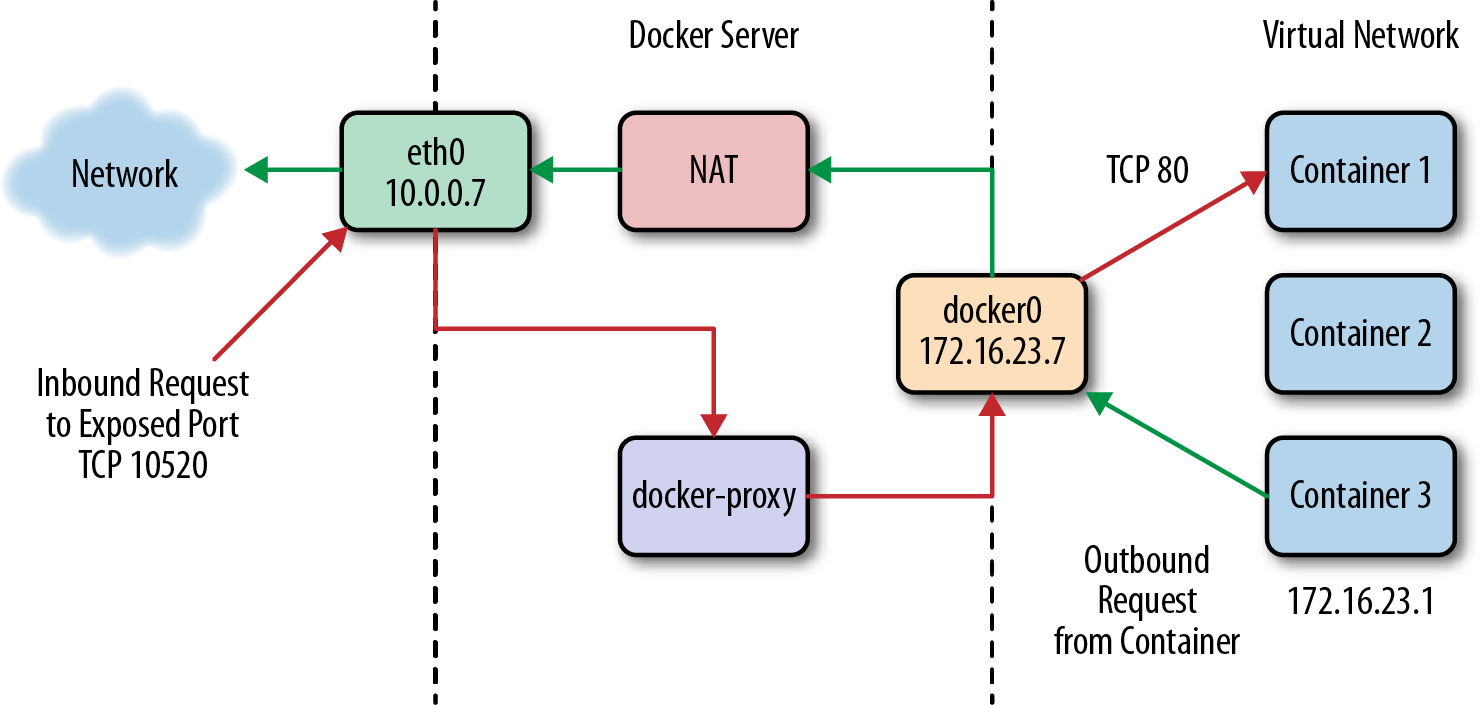
\includegraphics[width=.6\textwidth]{demo/img/swarm-network}
    \caption{Docker ma sieć\cite{docker_compose_reference}.}  \label{rys:network}
    % Źródło rysunku i~etykieta przez którą odwołujemy się do rysunku.
\end{figure}

Jak widać na rys. \ref{rys:network} Docker ma wewnętrzną sieć. \lipsum[1]


\subsection{Rysunek z~kotem}

Jak widać na rys.\ref{rysunek:kot} Ala ma kota. \lipsum[9-10]

\begin{figure}[H]
    \centering
\includegraphics[width=.4\textwidth]{demo/img/kotek}
    \caption{Ala ma kota \source{\ownwork}.}\label{rysunek:kot}
\end{figure}

\subsection{Tabela}

Co uwzględniono w~tabeli \ref{tabela:coktoma}. \lipsum[13-15]

% Tabela. Nazwa tabeli u~góry.
\begin{table}[h!]
    \centering\caption{Co kto ma\cite{harel_rzecz_2008} (patrz też dodatek~\ref{app:dod1}) \label{tabela:coktoma}}
    \begin{tabular}{|l|l|l|}% wyrównanie kolumn tabeli -> l~c r~- do lewej, środka, do prawej
        \hline
        Ala & ma & kota \\
        \hline
        Ola & ma & psa \\
        \hline
        Ula & ma & małpę\\
        \hline
    \end{tabular}
\end{table}

\lipsum[19-20] Warto wspomnieć, że w\cite{aizawa_groundwater_2009} rzecz przedstawiona jest zupełnie inaczej. Poniższy wzór:

\begin{equation}
    \sum_{i=1}^{\infty}a_i
    \label{eq:mojWzor}
\end{equation}

Wzór \ref{eq:mojWzor} wskazuje że dowód podany w\cite{kaleta_experimental_2005} może zostać podważony. \lipsum[9]

\section{Kod źródłowy}

% lub {java} albo {bash} albo {text}
\begin{listing}[h!]
    \begin{minted}{c}
        int main()
        {
        int a=2*3;
        printf("**Ala ma kota\n**");
        while(!I2C_CheckEvent(I2C1, I2C_EVENT_MASTER_MODE_SELECT)); /* EV5 */
        return 0;
        }
    \end{minted}
    \caption{Przykładowy algorytm w~języku C~\source{\ownwork}} \label{listing:moj}
\end{listing}

W~moim kodzie \ref{listing:moj} zrobiłem coś wspaniałego. \lipsum[4]

\thispagestyle{normal}

    % !TeX spellcheck = pl_PL
\chapter{Stan wiedzy i~techniki w~zakresie tematyki pracy}\label{ch:knowladge-state}
\section{Przegląd istniejących rozwiązań konkurencyjnych}\label{sec:competitive-solutions}

\lipsum[5]

W~tabeli \ref{tabela:rozwiazania-konkurencyjne-funkcjonalne} przedstawiono porównanie najważniejszych cech funkcjonalnych
istniejących na rynku rozwiązań konkurencyjnych.

\begin{minipage}{\textwidth}
    \begin{table}[H]
        \centering\caption{Rozwiązania konkurencyjne~- cechy funkcjonalne \source{\ownwork}\label{tabela:rozwiazania-konkurencyjne-funkcjonalne}}
        \begin{tabular}{|P{.22\textwidth}|P{.09\textwidth}|P{.09\textwidth}|P{.09\textwidth}|P{.09\textwidth}|P{.09\textwidth}|P{.09\textwidth}|}
            \hline
                                               & \cellgray{Rozw1}      & \cellgray{Rozw2}          & \cellgray{Rozw3}         & \cellgray{Rozw4}           & \cellgray{Rozw5}      & \cellgray{Rozw6}    \\ \hline
            \cellgray{Funkcjonalność 1}        & \cellgreen{TAK}       & \cellgreen{TAK}           & \cellgreen{TAK}          & \cellgreen{TAK}            & \cellgreen{TAK}       & \cellgreen{TAK}     \\ \hline
            \cellgray{Funkcjonalność 2}        & \cellgreen{TAK}       & \cellgreen{TAK}           & \cellgreen{TAK}          & \cellgreen{TAK}            & \cellred{NIE}         & \cellred{NIE}       \\ \hline
            \cellgray{Funkcjonalność 3}        & \cellgreen{TAK}       & \cellgreen{TAK}           & \cellgreen{TAK}          & \cellgreen{TAK}            & \cellgreen{TAK}       & \cellgreen{TAK}     \\ \hline
            \cellgray{Funkcjonalność 4}        & \cellgreen{TAK}       & \cellgreen{TAK}           & \cellgreen{TAK}          & \cellgreen{TAK}            & \cellred{NIE}         & \cellgreen{TAK}     \\ \hline
            \cellgray{Funkcjonalność 5}        & \cellgreen{TAK}       & \cellgreen{TAK}           & \cellgreen{TAK}          & \cellred{NIE}              & \cellred{NIE}         & \cellgreen{TAK}     \\ \hline
            \cellgray{Funkcjonalność 6}        & \cellgreen{TAK}       & \cellgreen{TAK}           & \cellgreen{TAK}          & \cellgreen{TAK}            & \cellgreen{TAK}       & \cellgreen{TAK}     \\ \hline
            \cellgray{Funkcjonalność 7}        & \cellgreen{TAK}       & \cellgreen{TAK}           & \cellgreen{TAK}          & \cellred{NIE}              & \cellgreen{TAK}       & \cellgreen{TAK}     \\ \hline
            \cellgray{Funkcjonalność 8}        & \cellgreen{TAK}       & \cellgreen{TAK}           & \cellgreen{TAK}          & \cellgreen{TAK}            & \cellgreen{TAK}       & \cellred{NIE}       \\ \hline
            \cellgray{Funkcjonalność 9}        & \cellgreen{TAK}       & \cellgreen{TAK}           & \cellgreen{TAK}          & \cellgreen{TAK}            & \cellgreen{TAK}       & \cellgreen{TAK}     \\ \hline
            \cellgray{Funkcjonalność 10}       & \cellgreen{TAK}       & \cellgreen{TAK}           & \cellgreen{TAK}          & \cellgreen{TAK}            & \cellgreen{TAK}       & \cellgreen{TAK}     \\ \hline
        \end{tabular}
    \end{table}
\end{minipage}

\section{Przegląd literatury domenowej}\label{sec:domain-literature}

\lipsum[5]

\section{Przegląd przydatnych technologii}\label{sec:usefull-technologies}

\lipsum[5]

\thispagestyle{normal}

    % !TeX spellcheck = pl_PL
\chapter{Założenia projektowe}\label{ch:design-assumptions}
\section{Uwagi wstępne}\label{sec:presumptions}

\lipsum[5]

\section{Słownik pojęć domenowych}\label{sec:dictionary}

Na podstawie rozważań z~rozdziału \ref{ch:knowladge-state} sporządzono następującą listę definicji domenowych istotną z~punktu widzenia projektu:
\begin{itemize}[series=atr, wide, align=left, leftmargin=190pt]
    \atr{BIA}- metoda impedancji bioelektrycznej wykorzystywana do analizy składu ciała
    \atr{BMI}- wskaźnik masy ciała
    \atr{CPM}- całkowita przemiana materii
\end{itemize}

\section{Sformułowanie problemu}\label{sec:problem-specification}

\par
W~tabeli \ref{tabela:sformulowanie-problemu} przedstawiono sformułowanie rozważanego w~pracy problemu wraz z~jego wpływem i~propozycją pomyślnego rozwiązania.

\begin{minipage}{\textwidth}
    \begin{table}[H]
        \centering\caption{Sformułowanie problemu \source{\ownwork}\label{tabela:sformulowanie-problemu}}
        \begin{tabular}{|P{.2\textwidth}|p{.7\textwidth}|}

            \hline
            \cellgray{Problem} &
            \inlinetodo{todo} \\
            \hline

            \cellgray{Dotyczy} &
            \inlinetodo{todo} \\
            \hline

            \cellgray{Wpływ problemu} &
            \begin{itemize}
                \item \inlinetodo{todo}
                \item \inlinetodo{todo}
                \item \inlinetodo{todo}
            \end{itemize} \\
            \hline

            \cellgray{Pomyślne rozwiązanie} &
            \begin{itemize}
                \item \inlinetodo{todo}
                \item \inlinetodo{todo}
                \item \inlinetodo{todo}
            \end{itemize} \\
            \hline
        \end{tabular}
    \end{table}
\end{minipage}

\pagebreak
\section{Pozycjonowanie produktu}\label{sec:product-positioning}

\par
W~tabeli \ref{tabela:pozycjonowanie-produktu} przedstawiono pozycjonowanie opracowywanego produktu względem rynku produktów z dziedziny.

\begin{minipage}{\textwidth}
    \begin{table}[H]
        \centering\caption{Pozycjonowanie produktu \source{\ownwork}\label{tabela:pozycjonowanie-produktu}}
        \begin{tabular}{|P{.2\textwidth}|p{.7\textwidth}|}

            \hline
            \cellgray{Dla} &
            \inlinetodo{todo} \\
            \hline

            \cellgray{Który} &
            \inlinetodo{todo} \\
            \hline

            \cellgray{Nazwa produktu} &
            \inlinetodo{todo} \\
            \hline

            \cellgray{Który} &
            \inlinetodo{todo} \\
            \hline

            \cellgray{Inaczej niż} &
            \inlinetodo{todo} \\
            \hline

            \cellgray{Nasz produkt} &
            \inlinetodo{todo} \\
            \hline
        \end{tabular}
    \end{table}
\end{minipage}

\pagebreak
\section{Podsumowanie użytkowników systemu}\label{sec:users-summary}
\par
W~tabeli \ref{tabela:uzytkownicy} przedstawiono podsumowanie użytkowników projektowanego systemu, ich krótki opis oraz ich podstawowe odpowiedzialności związane z~korzystaniem z~systemu.

\begin{minipage}{\textwidth}
    \begin{table}[H]
        \centering\caption{Użytkownicy \source{\ownwork}\label{tabela:uzytkownicy}}
        \begin{tabular}{|P{.15\textwidth}|P{.25\textwidth}|P{.5\textwidth}|}

            \hline
            \cellgray{Nazwa} & \cellgray{Opis} & \cellgray{Odpowiedzialności}\\

            \hline
            Gość &
            Niezalogowany użytkownik &
            \begin{itemize}
                \item Zakłada konto użytkownika.
                \item Wyświetla stronę główną.
            \end{itemize} \\
            \hline
            Administrator &
            Osoba zarządzająca działaniem aplikacji &
            \begin{itemize}
                \item Przydzielanie i~odbieranie użytkownikom uprawnień.
                \item Zarządzanie definicjami wartości odżywczych, typami diet, typami posiłków, typami dań i~wyposażeniem kuchennym.
            \end{itemize} \\
            \hline
        \end{tabular}
    \end{table}
\end{minipage}

\section{Wymagania funkcjonalne}\label{sec:functional-requirements}
\par
W~tabeli \ref{tabela:wymaganiaFunkcjonalne}
przedstawiono wymagania funkcjonalne dla systemu w~postaci zestawienia potrzeb użytkowników systemu z~cechami związanymi z~realizacją danej potrzeby.
Następnie wymagania sformalizowano w~postaci diagramów przypadków użycia języka UML na rysunku \ref{fig:use-case-diagram:gateway}.

\begin{minipage}{\textwidth}
    \begin{table}[H]
        \centering\caption{Wymagania funkcjonalne \source{\ownwork}\label{tabela:wymaganiaFunkcjonalne}}
        \begin{tabular}{|P{.3\textwidth}|P{.6\textwidth}|}
            \hline
            \cellgray{Potrzeby} & \cellgray{Cechy} \\

            \hline
            Administrator potrzebuje widzieć listę użytkowników &
            \begin{itemize}
                \item Przydzielanie i~odbieranie użytkownikom uprawnień.
            \end{itemize} \\
            \hline
            Użytkownik potrzebuje korzystać ze swojego konta &
            \begin{itemize}
                \item Logowanie do systemu.
                \item Przypomnienie hasła.
                \item Zarządzanie swoimi danymi osobowymi.
            \end{itemize} \\
            \hline
            Użytkownik chce przeglądać witrynę w~swoim języku &
            \begin{itemize}
                \item Obsługa witryny w~wielu językach.
            \end{itemize} \\
            \hline
            Gość potrzebuje korzystać z~systemu &
            \begin{itemize}
                \item Zakładanie konta użytkownika.
                \item Wyrażenie zgody na przetwarzanie swoich danych osobowych.
            \end{itemize} \\
            \hline
        \end{tabular}
    \end{table}
\end{minipage}

%\image{0.7}{img/gateway.png}{Diagram przypadków użycia}{use-case-diagram:gateway}

\newpage

\section{Wymagania niefunkcjonalne}\label{sec:nonfunctional-requirements}
\begin{itemize}
    \item System działa poprawnie w~przeglądarkach Google~Chrome~76, Mozilla~Firefox~69 i~Opera~63.
    \item System działa na urządzenia mobilnych korzystających z~systemu Android~9 i~iOS~12.
    \item System jest dostępny w~polskiej i~angielskiej wersji językowej.
    \item System ma czytelny i~minimalistyczny interfejs.
    \item Aplikacja webowa jest w~pełni responsywna i~wygodna do używania na ekranach od~5 do~30 cali.
\end{itemize}
\thispagestyle{normal}


    % !TeX spellcheck = pl_PL
\chapter{Projekt}\label{ch:project}

\section{Prototyp interfejsu}\label{sec:mockups}

\lipsum[5]

\section{Opis podstawowej architektury systemu}\label{sec:basicArchitecture}

\lipsum[5]

\section{Projekt bazy danych}\label{sec:database}

\subsection{Kategorie}\label{subsec:database:categories}

\begin{enumerate}[label={\textbf{KAT/\protect\threedigits{\theenumi}}}, wide, labelwidth=!, labelindent=0pt, labelsep=0pt, series=reqs]
    \setlength\itemsep{1.75em}
    \req{User}\label{kat:User} (Użytkownik)\\
    \indent\textbf{Opis}: Konto użytkownika aplikacji. Każdy zalogowany użytkownik musi mieć konto użytkownika.
    \par
    \textbf{Atrybuty}:
    \begin{itemize}[series=atr, wide, align=left, leftmargin=190pt]
        \atr{id}\label{kat:User:id}- identyfikator
        \atr{login}\label{kat:User:login}- login użytkownika
        \atr{passwordHash}\label{kat:User:passwordHash}- reprezentacja hasła utworzona przez nałożenie na hasło funkcji skrótu
    \end{itemize}

    \req{Authority}\label{kat:Authority} (Rola)\\
    \indent\textbf{Opis}: Rola użytkownika od której zależy zakres uprawnień użytkownika.
    \par
    \textbf{Atrybuty}:
    \begin{itemize}[series=atr, wide, align=left, leftmargin=190pt]
        \atr{name}\label{kat:Authority:name}- nazwa roli
    \end{itemize}
\end{enumerate}

\subsection{Reguły funkcjonowania}\label{subsec:database:functionalRules}

\begin{itemize}[label={\textbf{Reguły dla}}, wide, labelwidth=!, labelindent=0pt]
    \setlength\itemsep{1.75em}
    \item\ref{kat:User}\mynobreakpar
    \begin{enumerate}[label={\textbf{REG/\protect\threedigits{\arabic{enumi}}}}, wide, labelwidth=!, align=left, leftmargin=3cm]
        %Relacje
        \item Użytkownik (\ref{kat:User}) musi mieć przynajmniej jedną rolę (\ref{kat:Authority}).
        \item Użytkownik (\ref{kat:User}) może mieć wiele ról (\ref{kat:Authority}).
        %CRUD
        \item \role{Gość} może dodawać nowego użytkownika (\ref{kat:User}).
        \item \role{Użytkownik} może wyświetlać, edytować i~usuwać swoje dane użytkownika (\ref{kat:User}).
        \item \role{Administrator} może wyświetlać i~usuwać dane użytkownika (\ref{kat:User}).
    \end{enumerate}
    \item\ref{kat:Authority}\mynobreakpar
    \begin{enumerate}[label={\textbf{REG/\protect\threedigits{\arabic{enumi}}}}, wide, labelwidth=!, align=left, leftmargin=3cm, resume]
        %Relacje
        %CRUD
        \item \role{Administrator} może dodawać, wyświetlać, edytować i~usuwać dane roli (\ref{kat:Authority}).
    \end{enumerate}
\end{itemize}

\subsection{Ograniczenia dziedzinowe}\label{subsec:database:restrictions}

\begin{itemize}[label={\textbf{Ograniczenia dla}}, wide, labelwidth=!, labelindent=0pt]
    \setlength\itemsep{1.75em}
    \item\ref{kat:User}\mynobreakpar
    \begin{enumerate}[label={\textbf{OGR/\protect\threedigits{\arabic{enumi}}}}, wide, labelwidth=!, align=left, leftmargin=3cm]
        %Required
        \item Atrybut \ref{kat:User:login} jest wymagany.
        \item Atrybut \ref{kat:User:passwordHash} jest wymagany.
        %Unique
        \item Atrybut \ref{kat:User:login} ma unikalną wartość.
        %Type
        \item Atrybut \ref{kat:User:login} jest ciągiem znaków składającym się z~liter, cyfr i~dodatkowo mogącym zawierać znaki ".", "\_", "-", "@" o~długości od 1~do 50 znaków.
        \item Atrybut \ref{kat:User:passwordHash} jest ciągiem znaków o~długości 60 znaków.
    \end{enumerate}
    \item\ref{kat:Authority}\mynobreakpar
    \begin{enumerate}[label={\textbf{OGR/\protect\threedigits{\arabic{enumi}}}}, wide, labelwidth=!, align=left, leftmargin=3cm, resume]
        \item Atrybut \ref{kat:Authority:name} jest wymagany.
        \item Atrybut \ref{kat:Authority:name} ma unikalną wartość.
        \item Atrybut \ref{kat:Authority:name} jest ciągiem znaków składającym się z~liter i~znaków "\_" o~długości od 1~do 255 znaków.
    \end{enumerate}

\end{itemize}

\subsection{Model informacyjny}\label{subsec:database:domainModel}

\lipsum[5]

\thispagestyle{normal}

    % !TeX spellcheck = pl_PL
\chapter{Implementacja}\label{ch:implementation}
\section{Wykorzystywane środowiska i~narzędzia programistyczne}\label{sec:dev-tools}

\lipsum[5]

\section{Zakres implementacji}\label{sec:implementation-scope}

\lipsum[5]

\section{Architektura systemu}\label{sec:system-architecture}

\lipsum[5]
\todo{diagram rozmieszczenia}

\subsection{Architektura backendu}\label{subsec:system-architecture:backend}

\lipsum[5]
\todo{diagram pakietów}

\subsection{Architektura frontendu}\label{subsec:system-architecture:frontend}

\lipsum[5]

\section{Dokumentacja kodu}\label{sec:code-documentation}

Podstawowa dokumentacja kodu została napisana przy użyciu komentarzy w~stylu kompatybilnym z~generatorem dokumentacji JavaDoc\cite{tech:javadoc}.
Przykładowy komentarz przedstawiono na listingu \ref{listing:javadoc}.

\noindent\hspace{.075\textwidth}\begin{minipage}{.85\textwidth}
    \begin{minted}{java}
/**
* Short description of measure.
*/
@NotNull
@Size(min = 1, max = 255)
private String description;
    \end{minted}
    \begin{lstlisting}[caption={Komentarz w~stylu JavaDoc \source{\ownwork}}, label={listing:javadoc}]
\end{lstlisting}
\end{minipage}

\section{Instalacja oprogramowania}\label{sec:software-installation}
\subsection{Wymagania wstępne}\label{subsec:prerequirements}

\lipsum[5]

\subsection{Instalacja}\label{subsec:installation}

\lipsum[5]

\section{Prezentacja aplikacji}\label{sec:app-presentation}

\lipsum[5]

\thispagestyle{normal}

    % !TeX spellcheck = pl_PL
\chapter{Testy}
\section{Wprowadzenie}

\lipsum[5]

\section{Testy jednostkowe}

\lipsum[5]

\section{Testy użyteczności}

\lipsum[5]

\thispagestyle{normal}


    % !TeX spellcheck = pl_PL
\chapter*{Zakończenie}\label{ch:ending}

W pracy udało mi się dużo zrobić. \lipsum[17]

\par
Mnóstwo innych rzeczy da się poprawić i rozwinąć. \lipsum[23]

\thispagestyle{normal}


    % W~pracy pojawią się tylko prace naprawdę cytowane.
    % \nocite{*}
    \cleardoublepage
    \bibliography{literatura}
    \bibliographystyle{dyplom}

    \listnormal{\listoffigures}{\listfigurename}
    \listnormal{\listoftables}{\listtablename}

    \clearpage
%    \listof{listing}{Spis kodów źródłowych}
    \lstlistoflistings

    % !TeX spellcheck = pl_PL
% \appendixpage
% \addappheadtotoc

\appendix
\begin{appendices}
    \chapter{To powinien być dodatek}\label{app:dod1}

    \lipsum[5]

\end{appendices}
\thispagestyle{normal}

\end{document}
